\beginsong{Kaspar}[wuw={Reinhard Mey, 1968}, pfii={94}, pfiii={45}, gruen={18}, kssiv={68}, siru={212}, index={Sie sagten, er käme von Nürnberg her}]

\beginverse
\endverse
\centering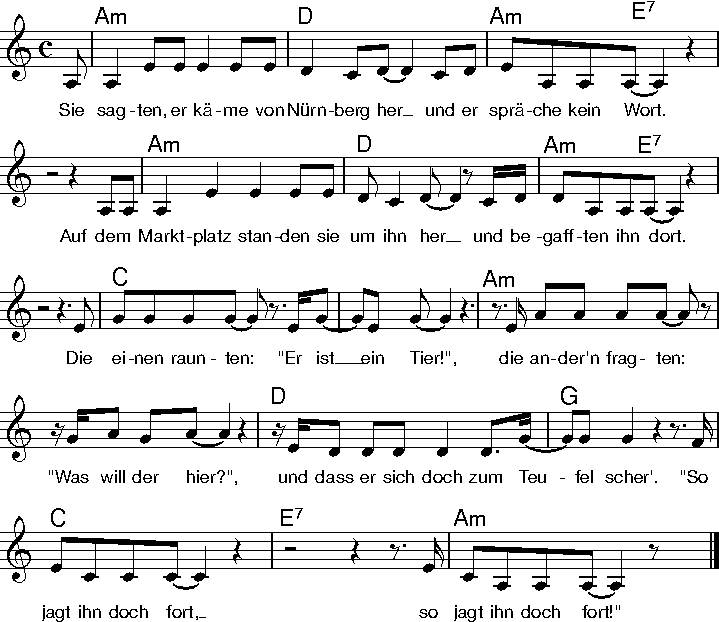
\includegraphics[width=1\textwidth]{Noten/Lied059.pdf}	

\beginverse\memorize
Sein \[Am]Haar in Strähnen und \[D]wirre, sein \[Am]Gang war gebeugt. \[E7]
''Kein \[Am]Zweifel, dieser \[D]Irre ward vom \[Am]Teufel gezeugt.'' \[E7]
Der \[C]Pfarrer reichte ihm einen Krug
voll \[Am]Milch, er sog ihn in einem Zug.
''\[D]Er trinkt nicht vom Ge\[G]schirre, 
den hat die \[C]Wölfin gesäugt,\[E7]  den hat die \[Am]Wölfin gesäugt.''
\endverse

\beginverse
Mein ^Vater, der in ^unserem Ort der ^Schulmeister war, ^
trat ^vor ihn hin, trotz ^böser Worte ^rings aus der Schar. ^
Er ^sprach zu ihm ganz ruhig und
der ^Stumme öffnete seinen Mund
^und stammelte die ^Worte
''Heiße ^Kaspar^, heiße ^Kaspar.''
\endverse 

\beginverse
Mein ^Vater brachte ^ihn ins Haus, ''^Heiße Kaspar.'' ^
Meine ^Mutter wusch ihm ^die Kleider aus ^und schnitt ihm das Haar. ^
Spre^chen lehrte mein Vater ihn,
^lesen und schreiben und es schien,
^was man ihn lehrte, sog ^er in sich auf,
wie ^gierig er war^, wie ^gierig er war.
\endverse

\beginverse
Zur ^Schule gehörte ^derzeit noch das ^Üttinger Feld. ^
Kaspar ^und ich, wir ^pflügten zu zweit, bald war ^alles bestellt. ^
Wir ^hegten und pflegten jeden Keim,
^brachten im Herbst die Ernte ein,
^von den Leuten vermale^deit,
von deren ^Hunden verbellt^, von deren ^Hunden verbellt.
\endverse

\beginverse
Ein ^Wintertag, der ^Schnee war frisch, ^es war Januar. ^
^Meine Mutter rief: ''^Kommt zu Tisch, ^das Essen ist gar.'' ^
Mein ^Vater sagte: ''Appetit'',
ich ^wartete auf Kaspars Schritt,
^mein Vater fragte ^mürrisch: 
''Wo bleibt ^Kaspar^, wo bleibt ^Kaspar?''
\endverse

\beginverse
Wir ^suchten und wir ^fanden ihn auf dem ^Pfad bei dem Feld. ^
Der ^Neuschnee wehte ^über ihn, ^sein Gesicht war entstellt, ^
die ^Augen angstvoll aufgerissen,
^sein Hemd war blutig und zerrissen.
^Erstochen hatten sie ^ihn 
dort am ^Üttinger Feld^, dort am ^Üttinger Feld.
\endverse

\beginverse
Der ^Polizeirat ^aus der Stadt füllte ^ein Formular. ^
''Gott ^nehm' ihn hin in ^seiner Gnad'', sagte ^der Herr Vikar. ^
Das ^Üttinger Feld liegt lang schon brach,
^nur manchmal bell'n mir noch die Hunde nach,
^dann streu' ich ein paar Blumen auf den ^Pfad 
für ^Kaspar^, für ^Kaspar.
\endverse

\endsong

\beginscripture{}
Die Geschichte um Kaspar Hauser (ca. 1812 bis 1833) existiert in vielen verschiedenen Formen. Die Legende besagt, dass er in einer abgedunkelten Zelle von der Außenwelt abgeschnitten aufgezogen wurde, dabei standen ihm nur Grundnahrungsmittel zur Verfügung, sein Besitz umfasste die nötigste Kleidung und ein Schaukelpferd. Als 16-järiger tauchte er 1828 in Nürnberg auf. Daraufhin kursierten Gerüchte, dass Hauser aus dem badischen Fürstenhaus stamme. Der Rest wird in Reinhard Meys Lied erzählt.
\endscripture

\begin{intersong}
\ifthenelse{\boolean{pics}}{
    \ThisLRCornerWallPaper{0.8}{Bilder/IrenaRuppertirena_ruppert_Kaspar.png}
}{}
\end{intersong}